\subsection{Plot Determining Fixed Learning Rate to Use}
\begin{figure}
    \centering
    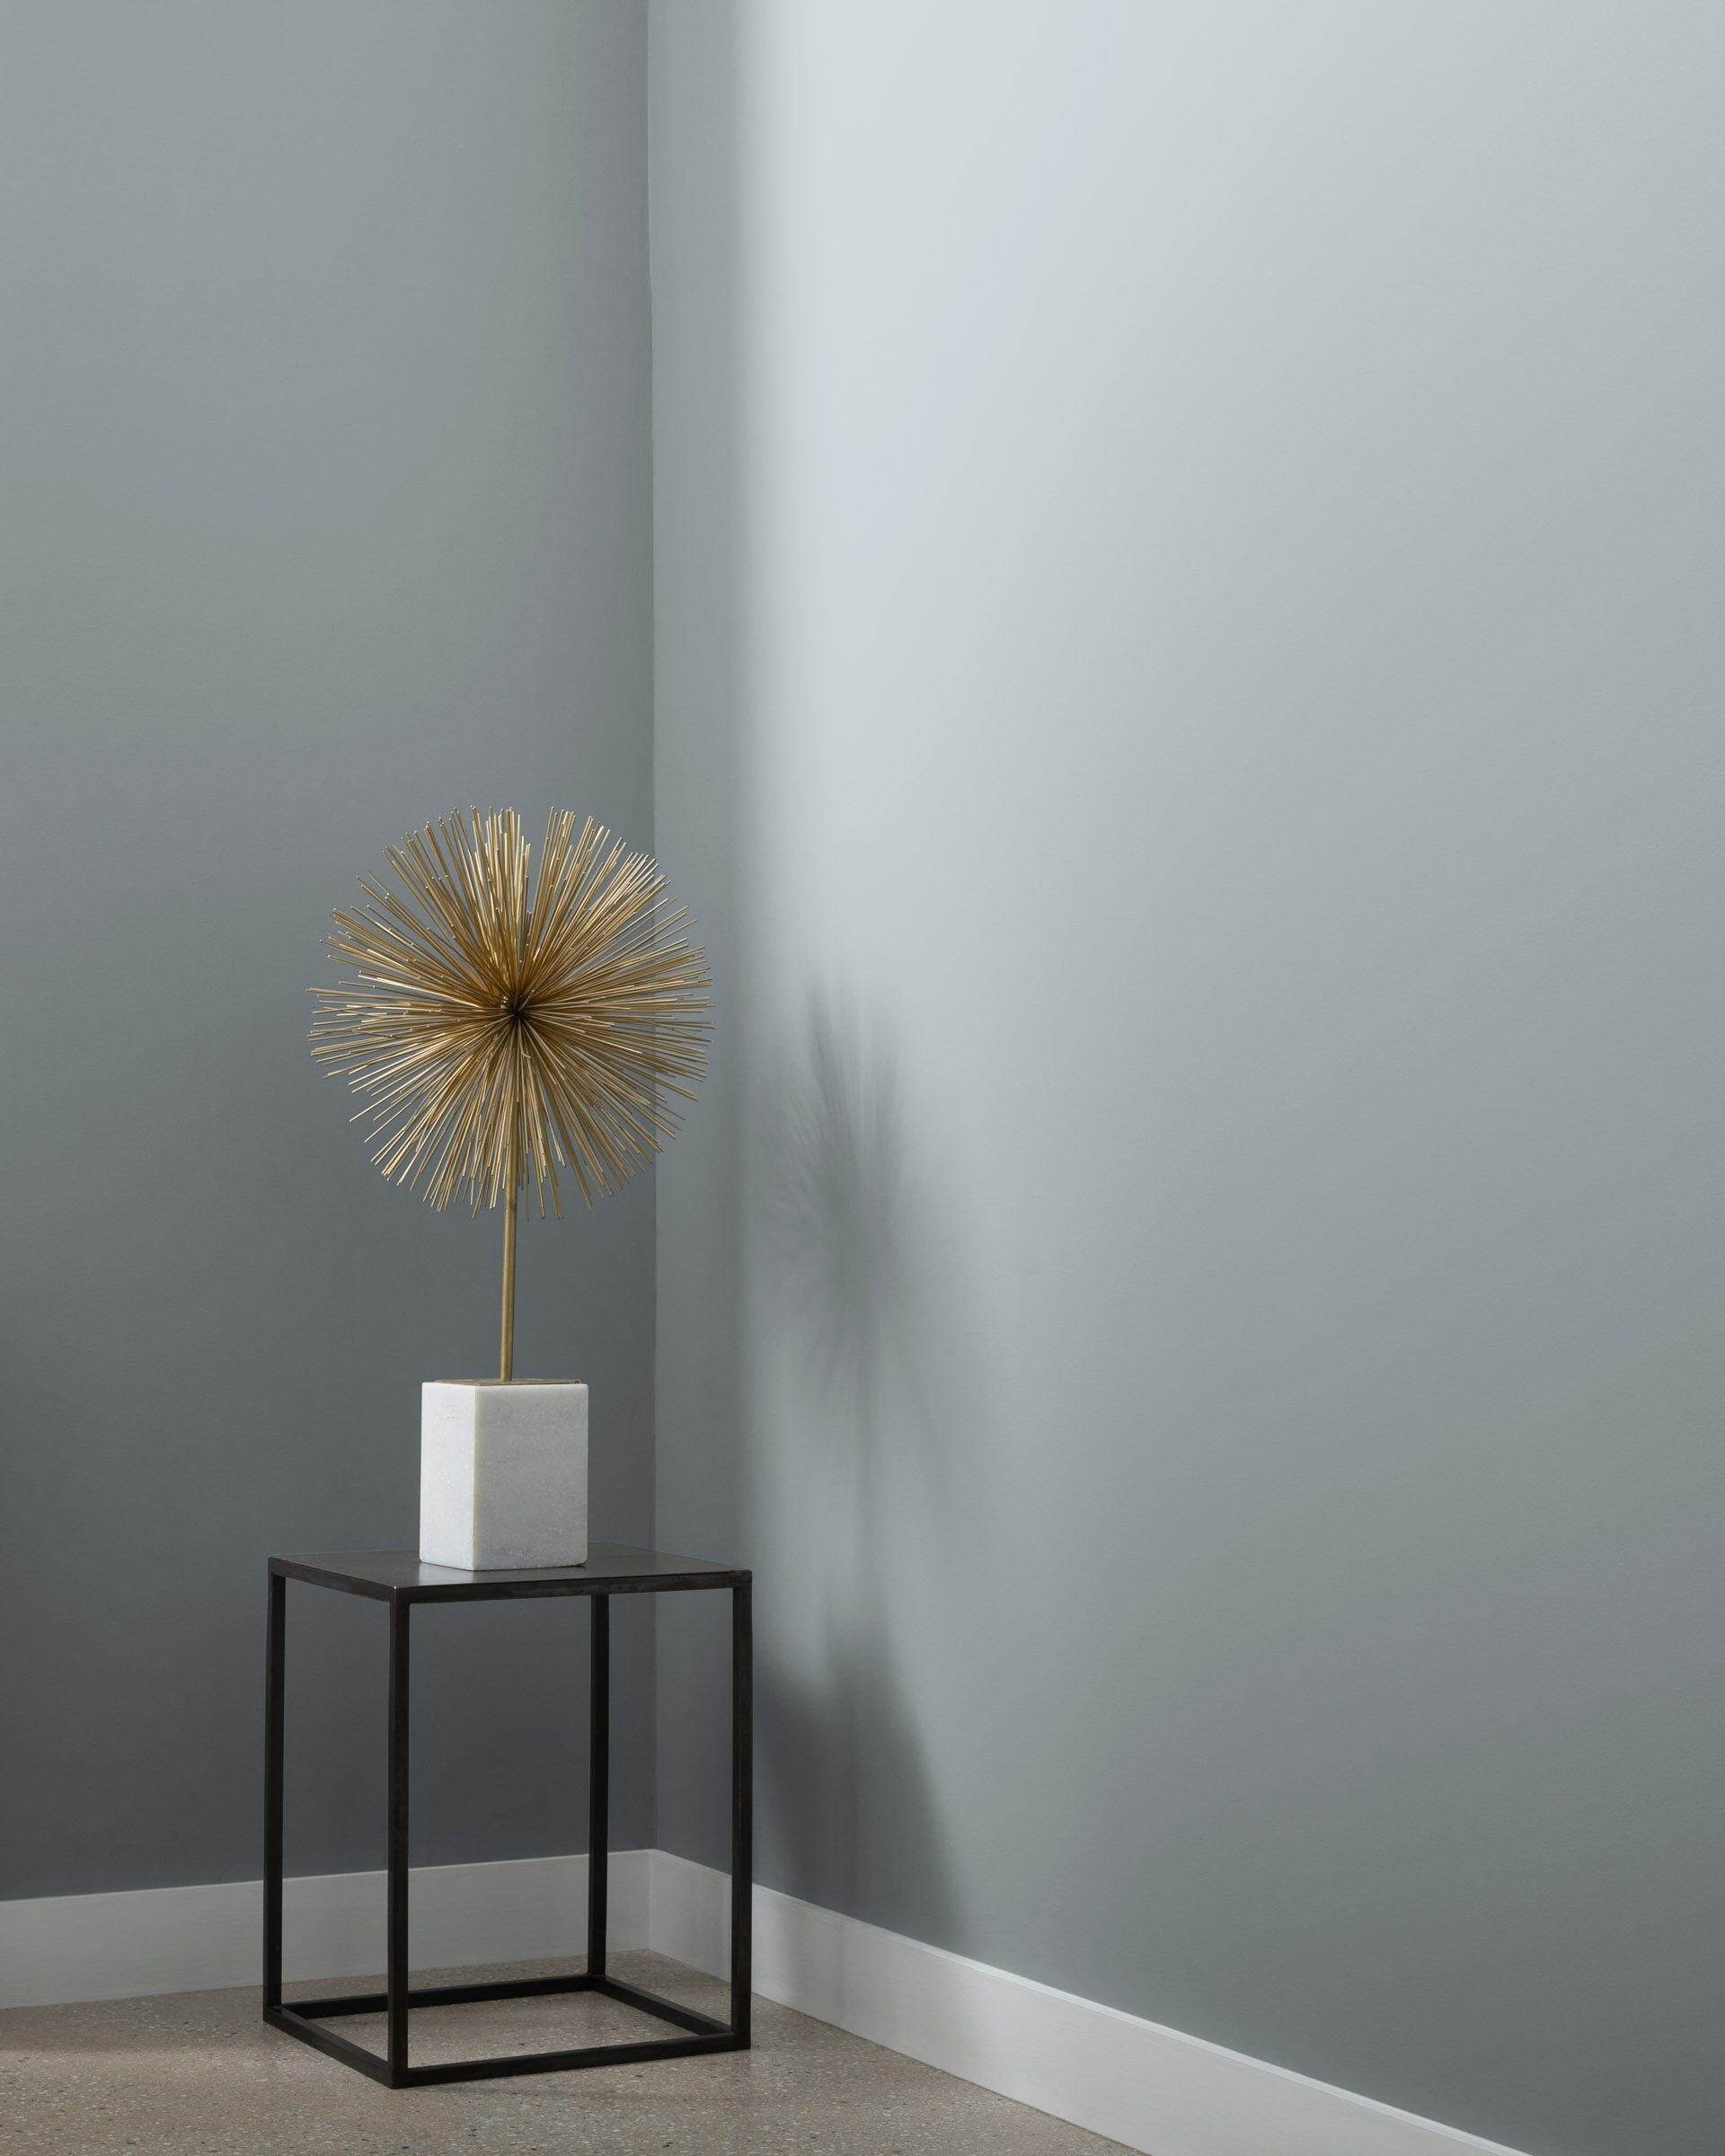
\includegraphics[width=0.5\linewidth]{figures/placeholders/plainWithDifferentLR.png}
    \caption{\textcolor{purple}{Plot showing our plain GD with 5 different learning rates as function of iterations.}}
    \label{fig:plainWithDifferentLR}
\end{figure}

\subsection{Grid Search Table Determining Best Hyperparameters for Ridge Regression with Respect to $R^2$ Score}
%Add figure code here if desired.

\subsection{$R^2$ Score of Experimentally-Determined Optimal Models}
\begin{figure}
    \centering
    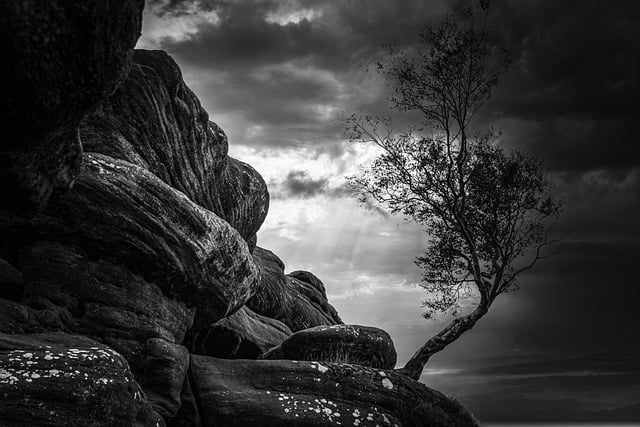
\includegraphics[width=0.5\linewidth]{figures/placeholders/numericalpredictionR2.png}
    \caption{\textcolor{purple}{$R^2$ score as a function of epochs for OLS, Ridge and neural network (optimal version of all three methods). We also need a sklearn comparison here.}}
    \label{fig:numericalpredictionR2}
\end{figure}